% Filename  : samplepaper.tex
% Purpose   : A sample exam paper to demonstrate how to use the 'ditpaper'
%             TeX class.
% Author    : Emmet Caulfield
% Revision  : $Id: samplepaper.tex 2 2006-02-19 20:34:45Z emmet $
% Repository: $HeadURL: http://svn.netrogen.lan/tex-ditpaper/trunk/samplepaper.tex $
%

% 'nosolution' (default) and 'solution' toggle the inclusion of solutions
% in the output. The tag nosolution, below, is replaced by 'sed' 
% in the Makefile to cause both the paper and the solutions to be produced.
\documentclass[nosolution]{ditpaper}
%\documentclass[solution]{ditpaper}


\usepackage{graphicx}
\usepackage{multirow}
\usepackage{rotating}


% These must be set or bizarre defaults will be used:
\facility{Kevin Street, Dublin 8}
\course{BSc. (Hons) in Computer Science}
\examcode{R228/419C}
\stage{Stage 4}
\session{Supplemental Examinations 2014}
\title{Artificial Intelligence II}
\examiners{Dr. John Kelleher\\
Dr. Deirdre. Lillis\\
Mr. P. Collins}
\examdate{}
\examtime{Duration: 2 Hours}
\instructions{Question 1 is \textbf{compulsory}\par{} Answer Question 1 (40 marks) \textbf{and}\par{} any 2 Other Questions (30 marks each).}


\begin{document}


%aima chapters 18
% inductive bias, learning theory - supervised/unsupervised, overfitting, lazy/eager learner, classification v regression, false positive v false negatives, linear separability, consistency, evaluation

\question
\begin{enumerate}
	\item Explain what is meant by \textbf{inductive learning}.
	\marks{5}
	\begin{answer}
		Inductive Learning involves the process of learning by example where a system tries to induce a general rule from a set of observed instances
	\end{answer}
\item Distinguish between \textbf{supervised} and \textbf{unsupervised} learning.
		\marks{5}
		\begin{answer}
			The distinction is that with \textbf{supervised learning} we know the actual label or category for each piece of data on which we train, whereas with \textbf{unsupervised learning} we do not know the classification of the data in the training sample. Unsupervised learning can thus often be viewed as a \textbf{clustering} task, while supervised learning can usually be seen as a \textbf{classification} task, or equivalently as a function-fitting task where one extrapolates the shape of a function based on some data points.
		\end{answer}

\item Distinguish between \textbf{classification learning} and \textbf{regression learning}.\\
\marks{5}
\begin{answer}
\begin{itemize}
\item learning a discrete-valued function is called classification learning
\item learning a continuous function is called regression.
\end{itemize}
\end{answer}
	\item In the context of inductive learning explain what is meant by a \textbf{consistent hypothesis}.
	\marks{5}
		\begin{answer}
		A hypothesis is consistent if it agrees with the true function on all examples that we have.
		\end{answer}
	\item  Inductive machine learning is often referred to as an \textbf{ill-posed problem}. What is meant by this?
	\marks{10}
	\begin{answer}
		Inductive machine learning algorithms essentially search through a hypothesis space to find a the best hypothesis that is consistent with the training data used. It is possible to find multiple hypotheses that are  consistent with a given training set (i.e. agrees with all training examples).  It is for this reason that inductive machine learning is referred to as an ill-posed problem as there is typically not enough information in the training data used to build a model to choose a single best hypothesis. Inductive machine learning algorithms must somehow choose one of the available hypotheses as the \emph{best}. An example like that shown in the figure below would be useful at this point
		\begin{center}
			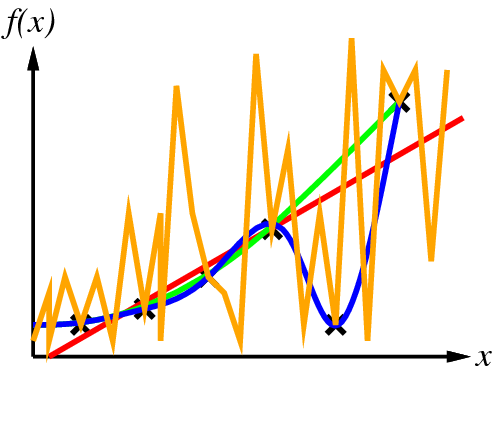
\includegraphics[width=5cm]{./images/curve-fitting5.png}
		\end{center}
	\end{answer}
\item Explain how do machine learning algorithms deal with the fact that machine learning is ill posed.
	\marks{10}
\begin{answer}
Because inductive learning is ill-posed, we have to make some extra assumptions to have a unique solution with the data we have. The set of assumptions we make to have learning possible is called the \textbf{inductive bias} of the learning algorithm - this is the main implication of inductive machine learning being ill-posed.\end{answer}




\end{enumerate}


\newpage

%Q2
% knn and CBR 
% information theory, entropy, Decision Trees, Inductive logic programming
		
\begin{table}[htdp]
\caption{Dataset for the 3-Nearest Neighbor question}
\begin{center}
\begin{tabular}{|c|c|c|c|}
\hline
ID & Feature1 & Feature2  & Target \\
\hline
101 & 4 &	180000 & C1\\
102 & 3 &	120000 & C2\\
103 & 7 &	360000 & C2\\
104 & 5 &	420000 &	C1\\
105 & 8 &	480000 &	C2\\
\hline
\end{tabular}
\end{center}
\label{tab:3nn-data}
\end{table}%

\begin{table}[htdp]
\caption{Query instance for the 3-Nearest Neighbor question.}
\begin{center}
\begin{tabular}{|c|c|c|c|}
\hline
ID & Feature1 & Feature2  & Target \\
\hline
250 & 4 &	240000 & ?\\
\hline
\end{tabular}
\end{center}
\label{tab:3nn-query}
\end{table}%
			
\question 
\begin{enumerate}
	\item Table \ref{tab:3nn-data} lists a dataset containing examples described by two descriptive features, \textbf{Feature1} and \textbf{Feature2}, and labelled with a target class \textbf{Target}. Table \ref{tab:3nn-query} lists the details of a query for which we want to predict  the target label. We have decided to use a \textbf{3-Nearest Neighbor} model for this prediction and we will use Euclidean distance as our distance metric: 
								\begin{center}
								$d(x_1,x_2)=\sqrt{\sum_{i=1}^{n} \left(\left(x_1.f_i - x_2.f_i \right)^2 \right)}$
								\end{center}					
		\begin{enumerate}
				\item What target class (\textbf{C1}  or \textbf{C2}) will our \textbf{3-Nearest Neighbor} model label the query with? Provide an explanation for you answer.				
			  \marks{5}
				\begin{answer}
					The first stage is to calculate the Euclidean distance between each of the examples and the query:
					\begin{center}
						\begin{tabular}{|c|c|}
						ID & Euclidean Distance \\
						\hline
						101 & 60000\\
						102 & 120000\\
						103 & 120000\\
						104 & 180000\\
						105 & 240000\\
						\hline
						\end{tabular}
					\end{center}
				 From this table we can see that the three closest examples to the query are examples 101, 102, and 103. Example 101 has a target label of C1 and both 102 and 103 have target labels C2. Consequently C2 is the majority label in local model constructed by the 3-Nearest Neighbor classifier for this query instance and the query will be labelled with class C2.
				\end{answer}
			\item There is a large variation in range between \textbf{Feature1} and \textbf{Feature2}. To account for this we decide to normalize the data. Compute the normalized data to four decimal points of precision using range normalization 
								\begin{center}
								$\displaystyle x_i.f^\prime=\frac{x_i.f - min(f)}{max(f)-min(f)}$
								\end{center}		
				\marks{5}
				\begin{answer}
					\begin{center}
\begin{tabular}{|c|c|c|c|}
\hline
ID & Feature1 & Feature2  & Target \\
\hline
101 &	0.2 &	 0.1667 &	C1\\
102 &	0    & 	0.0000 &	C2\\
103 &	0.8 & 	0.6667 &	C2\\
104 &	0.4 &	   0.8333 &	C1\\
105 &	1    & 	1.0000 &	C2\\
\hline
\end{tabular}
					\end{center}
				\end{answer}
			\item Assuming we use the normalized dataset as input, what target class (\textbf{C1}  or \textbf{C2}) will our \textbf{3-Nearest Neighbor} model label the query with? Provide an explanation for you answer.
			  \marks{5}
				\begin{answer}
					The normalize query instance is:
\begin{center}
\begin{tabular}{|c|c|c|c|}
\hline
ID & Feature1 & Feature2  & Target \\
\hline
250 & 0.2 & 0.3333 & ?\\
\hline
\end{tabular}
\end{center}
				The Euclidean distances between the normalized data and normalized query are: 
					\begin{center}
						\begin{tabular}{|c|c|}
						ID & Euclidean Distance \\
						\hline
101	& 0.1667\\
102	& 0.3887\\
103	& 0.6864\\
104	& 0.5385\\
105	&1.0414\\						
\hline
						\end{tabular}
					\end{center}
From this table we can see that the 3 closest neighbors are: 101, 103 and 104. 101 and 104 are both labelled as class \textbf{C1}. So \textbf{C1} is the majority class in the neighborhood and the query will be labelled as belonging to it.					
				\end{answer}	
		\end{enumerate}

		% Information theory and Decision Trees
		\item Table \ref{tab:id3data} (on the next page) lists a data set with of 6 examples described in terms of 3 binary descriptive features (\textbf{A}, \textbf{B}, and \textbf{C}) and a target feature (\textbf{Target}). You are asked to create a decision tree model using this data. \textbf{Which of the descriptive features will the ID3 decision tree induction algorithm choose as the feature for the root node of the decision tree?} Support you anwer with appropriate calculations and dicussions of your results. Note that Table \ref{tab:info-eqs} (also on the next page) lists some equations that you may find useful for this question.		
		\marks{15}
		\begin{answer}
		The ID3 decision tree induction algorithm selects the decriptive feature with the highest information gain as the feature for the root node of the decision tree.  The first step in calculating information gain is to calculate the entropy for the entire dataset:
	\begin{eqnarray*}
H\left(DS\right) &=& - \sum_{v \in \{C1,C2\}} p_v ~ log_2 p_v\\
		&=& -\left(\frac{3}{6}~ log_2 \frac{3}{6}\right) + -\left(\frac{3}{6} ~log_2 \frac{3}{6}\right)\\
		&=& 1.00~bits
	\end{eqnarray*}
	The table below shows the calculation of the infromation gain for each of the descriptive features in the dataset:
		\begin{scriptsize}
\begin{tabular}{ccccccc}
Split & Feature &              &  & Entropy of &  & Info.\\
By & Value & Partition  & Examples & Partition & Remainder & Gain\\
\hline
\multirow{2}{*}{A} & 1 & $DS_1$  & 1,2,3 & 0.9183 & \multirow{2}{*}{0.9183} & \multirow{2}{*}{0.0817}\\
 & 0 & $DS_2$ & 4,5,6 & 0.9183 &  & \\
\hline
\multirow{2}{*}{B} & 1 & $DS_3$ & 2,4,5,6 & 0.8113 & \multirow{2}{*}{0.5409} & \multirow{2}{*}{0.4591}\\
& 0 & $DS_4$ & 1,3 & 0 &  & \\
\hline
\multirow{2}{*}{C} & 1 & $DS_5$ & 1,2,3,4,6 & 0.9709 & \multirow{2}{*}{0.8091} & \multirow{2}{*}{0.1909}\\
& 0 & $DS_6$ & 5 & 0 &  & \\
\hline
\end{tabular}
	\end{scriptsize}
	From this table we can see the feature \textbf{B} has the highest information gain and consequently the ID3 algorithm will chose this feature as the feature tested at the root node of the tree.
		\end{answer}

\begin{table}[htb]
\centerline{
\begin{tabular}{|c|c|c|c|c|}
\hline
\textbf{ID}	 & \textbf{A}	& \textbf{B} & \textbf{C} & \textbf{Target}\\
\hline
1 & 1 & 0 & 1 & C1\\
2 & 1 & 1 & 1 & C2\\
3 & 1 & 0 & 1 & C1\\
4 & 0 & 1 & 1 & C2\\
5 & 0 & 1 & 0 & C1\\
6 & 0 & 1 & 1 & C2\\
\hline
\hline
\end{tabular}
}
\caption{Dataset for the ID3 Algorithm Question}
\label{tab:id3data}
\end{table}

	\begin{table}[htb]
	\begin{center}
	\begin{tabular}{rl}
	Entropy(DS) & $\displaystyle = -\sum_{i=1}^k p_i \times log_2(p_i)$\\
	Remainder(F) & $\displaystyle =\sum_{v \in Domain(F)} \frac{|DS_v|}{|DS|} Entropy(DS_v)$\\
	InformationGain(F,DS) & $\displaystyle =Entropy(DS)-Remainder(F)$\\
	\end{tabular}
	\end{center}
	\caption{Equations from information theory.}
	\label{tab:info-eqs}
	\end{table}


	\end{enumerate}

\clearpage
\newpage
	
%Q3 30 marks
% basic probability 5
% bayesian networks 10
% bayesian learning  15

\begin{table}[h]
\caption{Query Document}
\centering
\begin{tabular}{l}
\hline
\textit{Machine learning is fun}\\
\hline
\end{tabular}
\label{tab:likedislikequery}
\end{table}

\begin{table}[!htb]
    \caption{Document counts from the corpus for the words in the query.}
    \begin{minipage}{.5\linewidth}
      \centering
Document counts for the \textbf{dislike} data set
\begin{tabular}{|c|c|c|c|}
\hline
fun & is & machine & learning\\
415 & 695 & 35 & 70\\
\hline
\end{tabular}
    \end{minipage}%
    \begin{minipage}{.5\linewidth}
      \centering
Document counts for the \textbf{like} data set
\begin{tabular}{|c|c|c|c|}
\hline
fun & is & machine & learning\\
200 & 295 & 120 & 105\\
\hline
\end{tabular}
    \end{minipage} 
    \label{tab:doccounts}
\end{table}

\question Lets assume we are given a set of \textbf{700} training documents that a friend has classified as \textbf{dislike} and another \textbf{300} documents that they have classified as \textbf{like}. We are now given a new  document and asked to classify it. Table \ref{tab:likedislikequery} lists the content of this query document and Table \ref{tab:doccounts} gives the number of documents from each class (\textbf{dislike} and \textbf{like}) that the words in the query document occurred in. \textbf{What class will a \textbf{Naive Bayes} prediction model label the query document as belonging to?} (You must support your answer by showing the calculations that a Naive Bayes model will make.)
		\marks{30}
		\begin{answer}
			A Naive Bayes model will label the query with the class that has the highest probability under the assumption of conditional independence between the evidence features. So to answer this question we need to calculate the probability of each class given the evidence and assuming conditional independence across the evidence.\\
			To carry out these calculation we need to convert the raw documents counts into conditional probabilities by dividing each count by the total number of documents occuring in class:
\begin{center}
								\textbf{$P(w_k|C=dislike)$}
								\begin{tabular}{|c|c|c|c|}
								\hline
											$w_k$ & Count & $P(w_k | C=dislike)$\\
												\hline
								 fun & 415 & $\frac{415}{700} = .593$\\
								 			is & 695 & $\frac{695}{700} = .99$\\
											learning & 35 & $\frac{35}{700} = .05$\\
											machine & 70 & $\frac{70}{700} = .10$\\
								\hline
								\end{tabular}
\end{center}
\begin{center}
								\textbf{$P(w_k|C=like)$}										
								\begin{tabular}{|c|c|c|c|}
								\hline
								$w_k$ & Count & $P(w_k | C=like)$\\
												\hline
								 fun & 200 & $\frac{200}{300} = .667$\\
								 is & 295 & $\frac{295}{300} = .983$\\
								learning & 120 & $\frac{120}{300} = .40$\\
								machine & 105 & $\frac{105}{300} = .35$\\
								\hline
								\end{tabular}
\end{center}

We can now compute the probabilites of each class:\\

$P(dislike|Query~Document)$
			\begin{eqnarray*}
&=& P(dislike) \times P(Machine|dislike) \times P(learning|dislike) \times P(is|dislike) \times p(fun|dislike).\\
&=& 0.7 \times 0.593 \times 0.99 \times 0.5 \times 0.1\\
&=& 0.00205
			\end{eqnarray*}
$P(like|Query~Document)$
			\begin{eqnarray*}
&=& P(like) \times P(Machine|like) \times P(learning|like) \times P(is|like) \times p(fun|like).\\
&=& 0.3 \times 0.667 \times 0.983 \times 0.4 \times 0.35\\
&=& 0.00275
			\end{eqnarray*}
			
As $P(like|Query~Document) > P(dislike|Query~Document)$ the naive bayes classifier will return a label of \textbf{like}.
		\end{answer}
%
\newpage

%Q4
%Linear Regression Neural Nets, SVMs, Ensemble Learning
%Q4
%Linear Regression Neural Nets, SVMs, Ensemble Learning


\question 
	\begin{enumerate}
\question The following model is commonly used for continuous prediction tasks:

\begin{center}
$y(x)=w_0 + w_1x_1 + \dots + w_Dx_D$
\end{center}

\begin{enumerate}
\item Provide the name for this model and explain all of the terms that it contains.
\marks{5}

		\begin{answer}
		Students should explain that this is a simple linear regression model which can be effectively used to make predictions. $x$ is a vector of feature values for a query instance and $w$ is a vector of feature weights. An diagram of a simple one dimensional linear function would help.
		\end{answer}
				
\item Explain how the following model can overcome some of the limitations of the model given above. 
	\marks{8}

\begin{center}
$\displaystyle y(x)=\sum_{j=0}^{M - 1}w_j{\phi}_j(x)$
\end{center}
\end{enumerate} 

		\begin{answer}
		Students should explain that the simple linear regression model is attractive because it is linear with respect to $w$ but has severe limitations because it is also linear with respect to x. These greatly limits the kinds of predictions that this model will be able to make. However, the introduction of \emph{basis functions}, shown as $\phi$ above, goes some way towards solving this problem. The introduction of a non-linear basis function means that models can be made non-linear functions of input $x$ but remain linear in $w$ which makes them computationally easier to solve.
		
		Students might give the example of polynomial regression in which ${\phi}_j(x)=x^j$ or some other suitable example.
		\end{answer}
		
		%Neural Nets	
\item Explain why a \textbf{linear threshold perceptron} can represent the AND and OR functions but not the XOR function.
	\marks{7}
	\begin{answer}
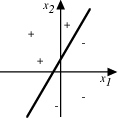
\includegraphics[width=1.5in]{./images/linear-separator.png}\\

We can think of a 2 input threshold perceptron as representing a line separator in 2D input space.In other words, the function $\sum_j W_j a_j > 0 \quad\mbox{or}\quad \vec{w} \bullet \vec{a} > 0$ defines a line in the input space and the perceptron outputs a 1 for instances lying on one side of the line and -1 for instances lying on the other side of the line.

The figure above illustrates this concept. The equation for the line in this image is $\vec{w} \bullet \vec{a} >0$. The inputs into the perceptron are $x_1$ and $x_2$; i.e. $\vec{a} = \{ x_1, x_2 \}$. 

This concept of a linear perceptron defining a line scales up into higher dimensional input space. In 3D and higher inputs space (i.e. in situations where the linear perceptron has 3 or more inputs), the linear activation function $\vec{w} \bullet \vec{a} >0$ defines a hyperplane decision surface in the $n$-dimensional space of inputs.

Data-sets of positive and negative examples that can be separated by a hyperplane are called \emph{linearly separabe}.

Of course, not all data-sets of positive and negative examples are linearly separable. The XOR function is one example of a non-linearly separable function. 

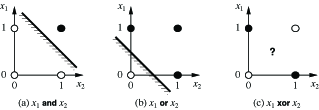
\includegraphics[width=3in]{./images/perceptron-linear.png}\\

The figure above illustrates this by comparing it with the AND and OR function which are linearly separable. In this figure black dots represent a point in the input space where the value of the function is 1, and white dots indicate a point where the value is 0.

As is evident from the images, in the AND and OR inputs spaces it is possible to draw a line that separates the black dots from the white dots. However, in the XOR space no such line exists. \emph{As a result, a threshold perceptron cannot represent the XOR function}.
	\end{answer}

\item Describe how perceptron training can be viewed as gradient descent search through an error landscape.
	\marks{10}
	\begin{answer}
Perceptrons learn by modifying the weights associated with their inputs in such a way as to minimize the error between the perceptrons output and the output expected by the training examples. 

As a result the set of possible weight vectors that the perceptron can adopt during training can be viewed as its hypothesis space. 	In the figure below the axes $w_0$ and $w_1$ represent possible values for two weights of a simple linear unit. The $w_0$, $w_1$ plane therefore represents the entire hypothesis space. 

Each position in this hypothesis space will have an associated error with. Mapping the error values as a error surface above the hypothesis allows us to view the error surface. In the figure below the the vertical axes indicates the error relative to some fixed set of training examples. The error surface shown in the figure thus summarises the desirability of every weight vector in the hypothesis space.

Perceptron learning adjusts the weights of the perceptron to minimise error. Consequently, it can be viewed as a gradient descent search for through the hypothesis space for the hypothesis (weight vector) with minimum error (i.e. the location in the hypothesis space whose associated error value is the global minimum in the error surface).

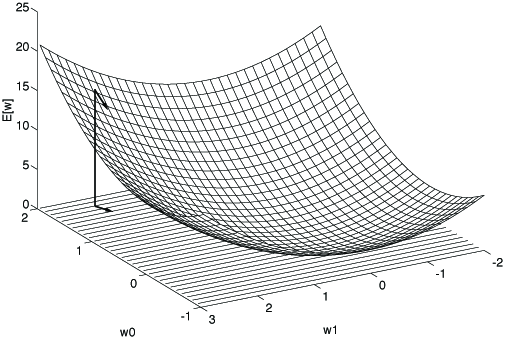
\includegraphics[width=3in]{./images/ann-hypothesis-space-and-error.png}
	
	\end{answer}
\end{enumerate}

\end{document}
